\subsection{Paper Prototype}\label{subsect:PaperPrototype}

The paper prototype was used to verify content placement and the number of actions required to complete the scenarios from Chapter 3 before visual details were introduced. At this stage we also identified recurring elements such as the header, bottom navigation, cards, status labels, calendar cells, and primary actions. The sketches are grouped by task below, following the same division later used in the digital prototype.

\paragraph{Common Screens}

The first sketches defined the shared authentication entry point and the two Home screens (Figure \ref{fig:paperCommonScreens}). Login and password recovery use the same structure for both roles, while the Home alternatives introduce the different priorities immediately after access: the member sees personal activities, whereas the professional sees the daily client agenda.

\begin{figure}[H]
    \centering
    \begin{subfigure}[c]{0.52\textwidth}
        \centering
        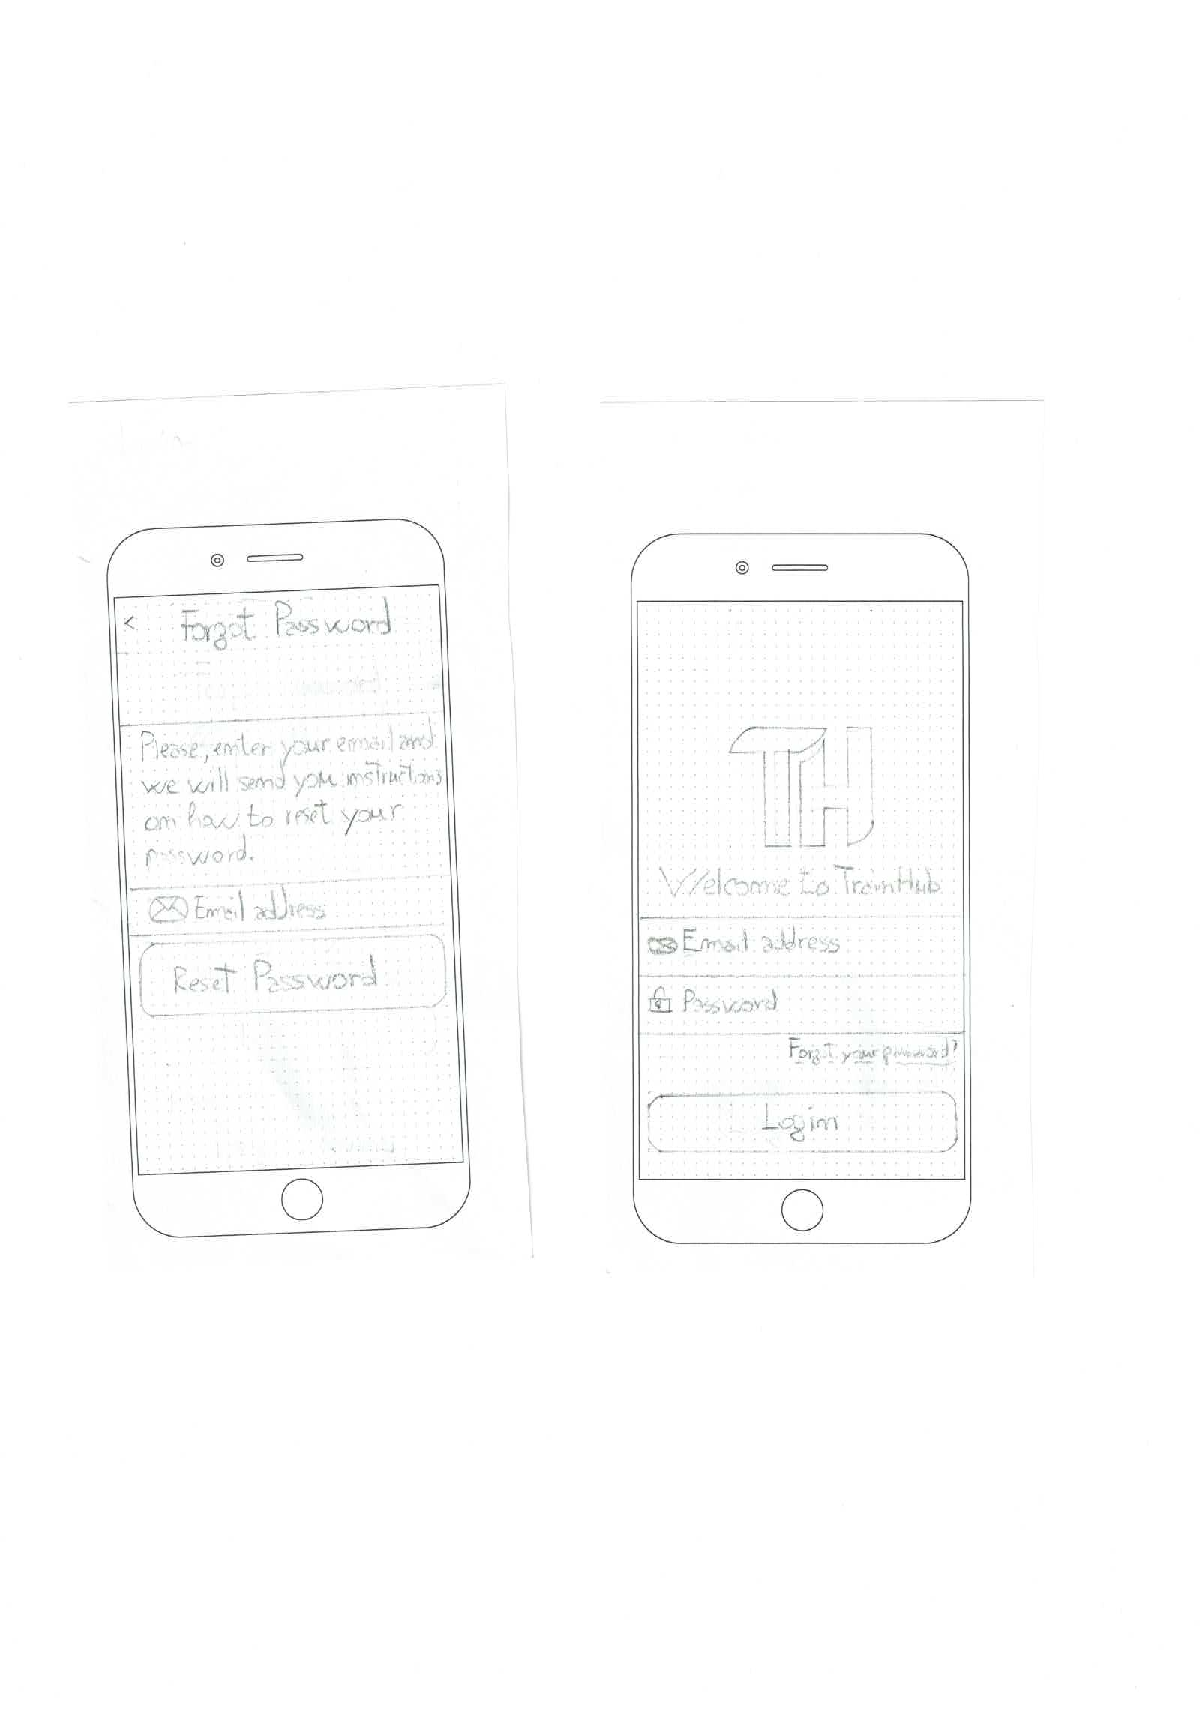
\includegraphics[width=\linewidth,trim=24bp 145bp 60bp 165bp,clip]{4-ApplicationDesign/img/PaperPrototype/paper-authentication.pdf}
        \caption{Authentication.}
    \end{subfigure}

    \vspace{0.35cm}
    \begin{subfigure}[c]{0.52\textwidth}
        \centering
        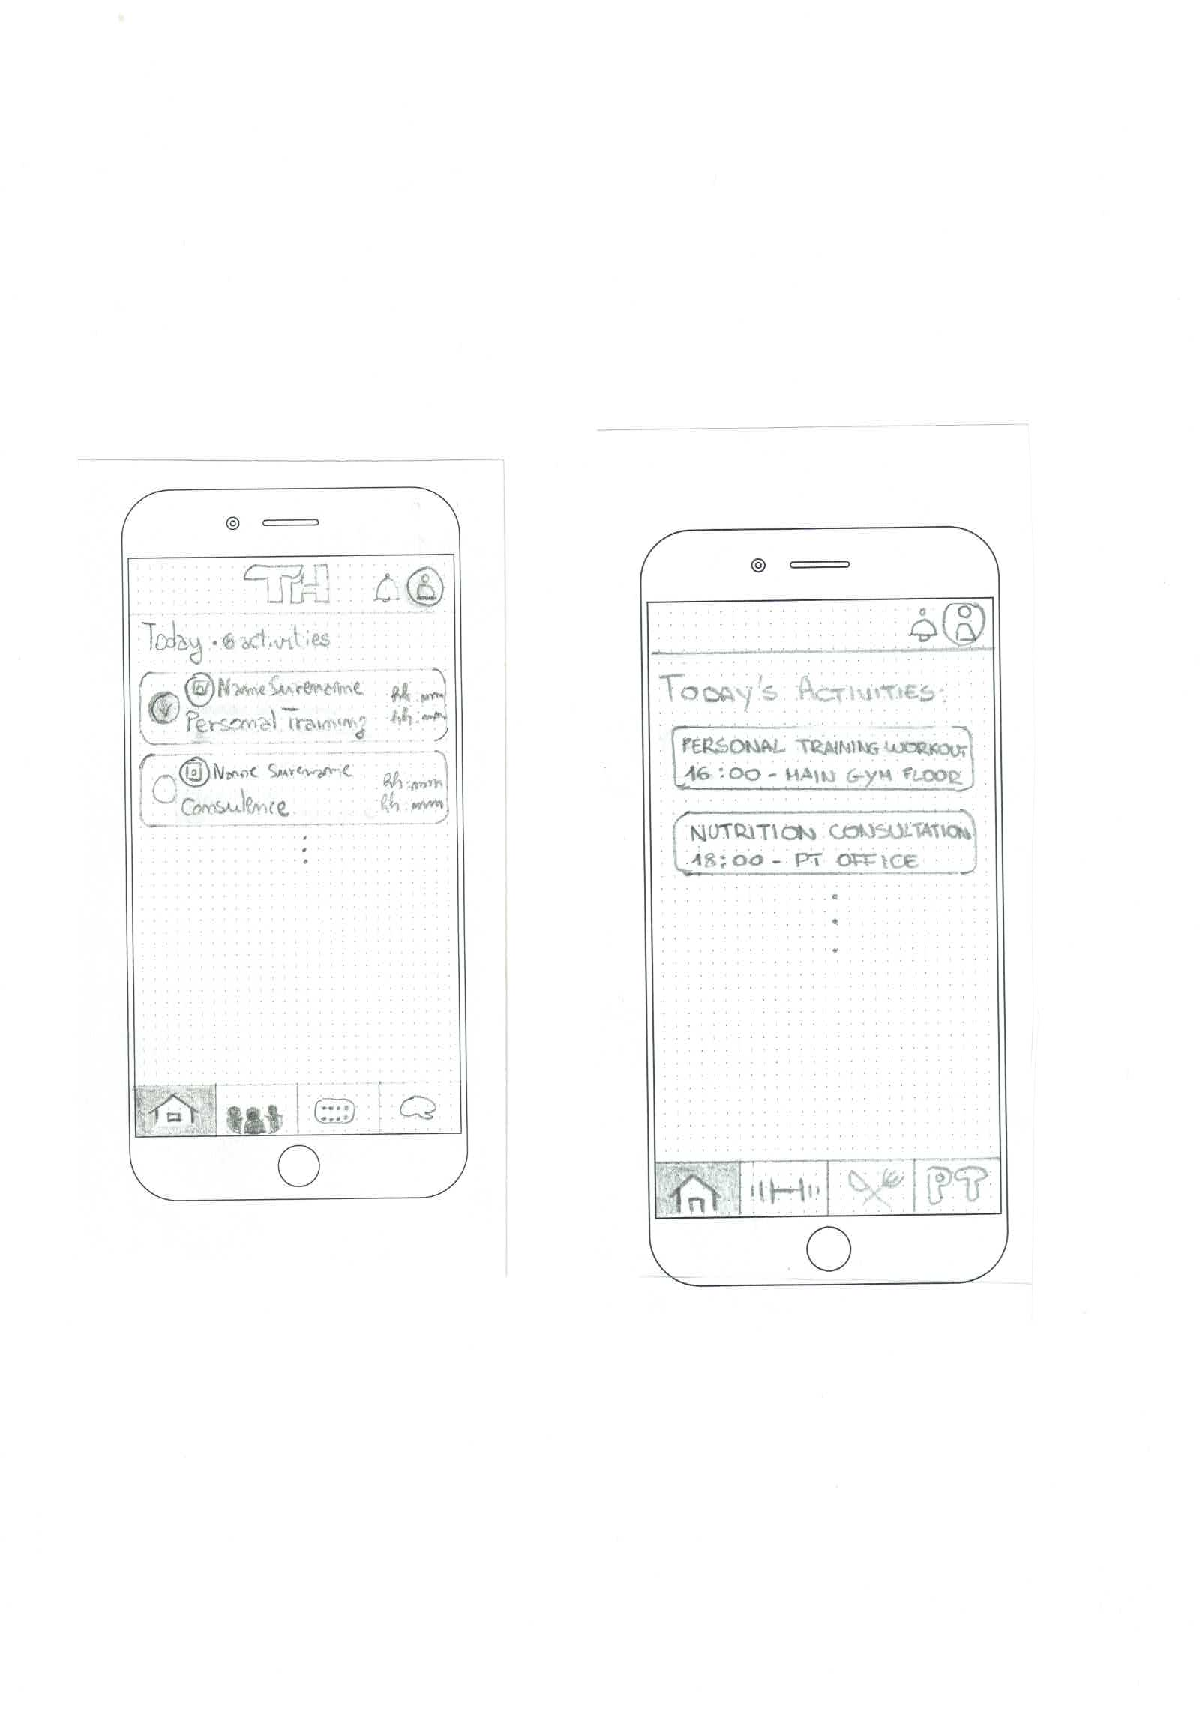
\includegraphics[width=\linewidth,trim=24bp 155bp 36bp 195bp,clip]{4-ApplicationDesign/img/PaperPrototype/paper-role-homes.pdf}
        \caption{Role-specific Home screens.}
    \end{subfigure}
    \caption{Shared entry screens in the paper prototype.}
    \label{fig:paperCommonScreens}
\end{figure}

\clearpage
\paragraph{Member Screens}

The member sketches were grouped around the four principal destinations. Workout moves from the plan list to session details and set recording (Figure \ref{fig:paperMemberWorkout}); Nutrition uses a shorter path from the assigned plan to its meals (Figure \ref{fig:paperMemberNutrition}). Personal Trainer combines professional selection, appointments, booking, and chat (Figures \ref{fig:paperMemberTrainer} and \ref{fig:paperMemberBooking}), while Profile collects access, subscription, and reward information (Figure \ref{fig:paperMemberProfile}).

\begin{figure}[H]
    \centering
    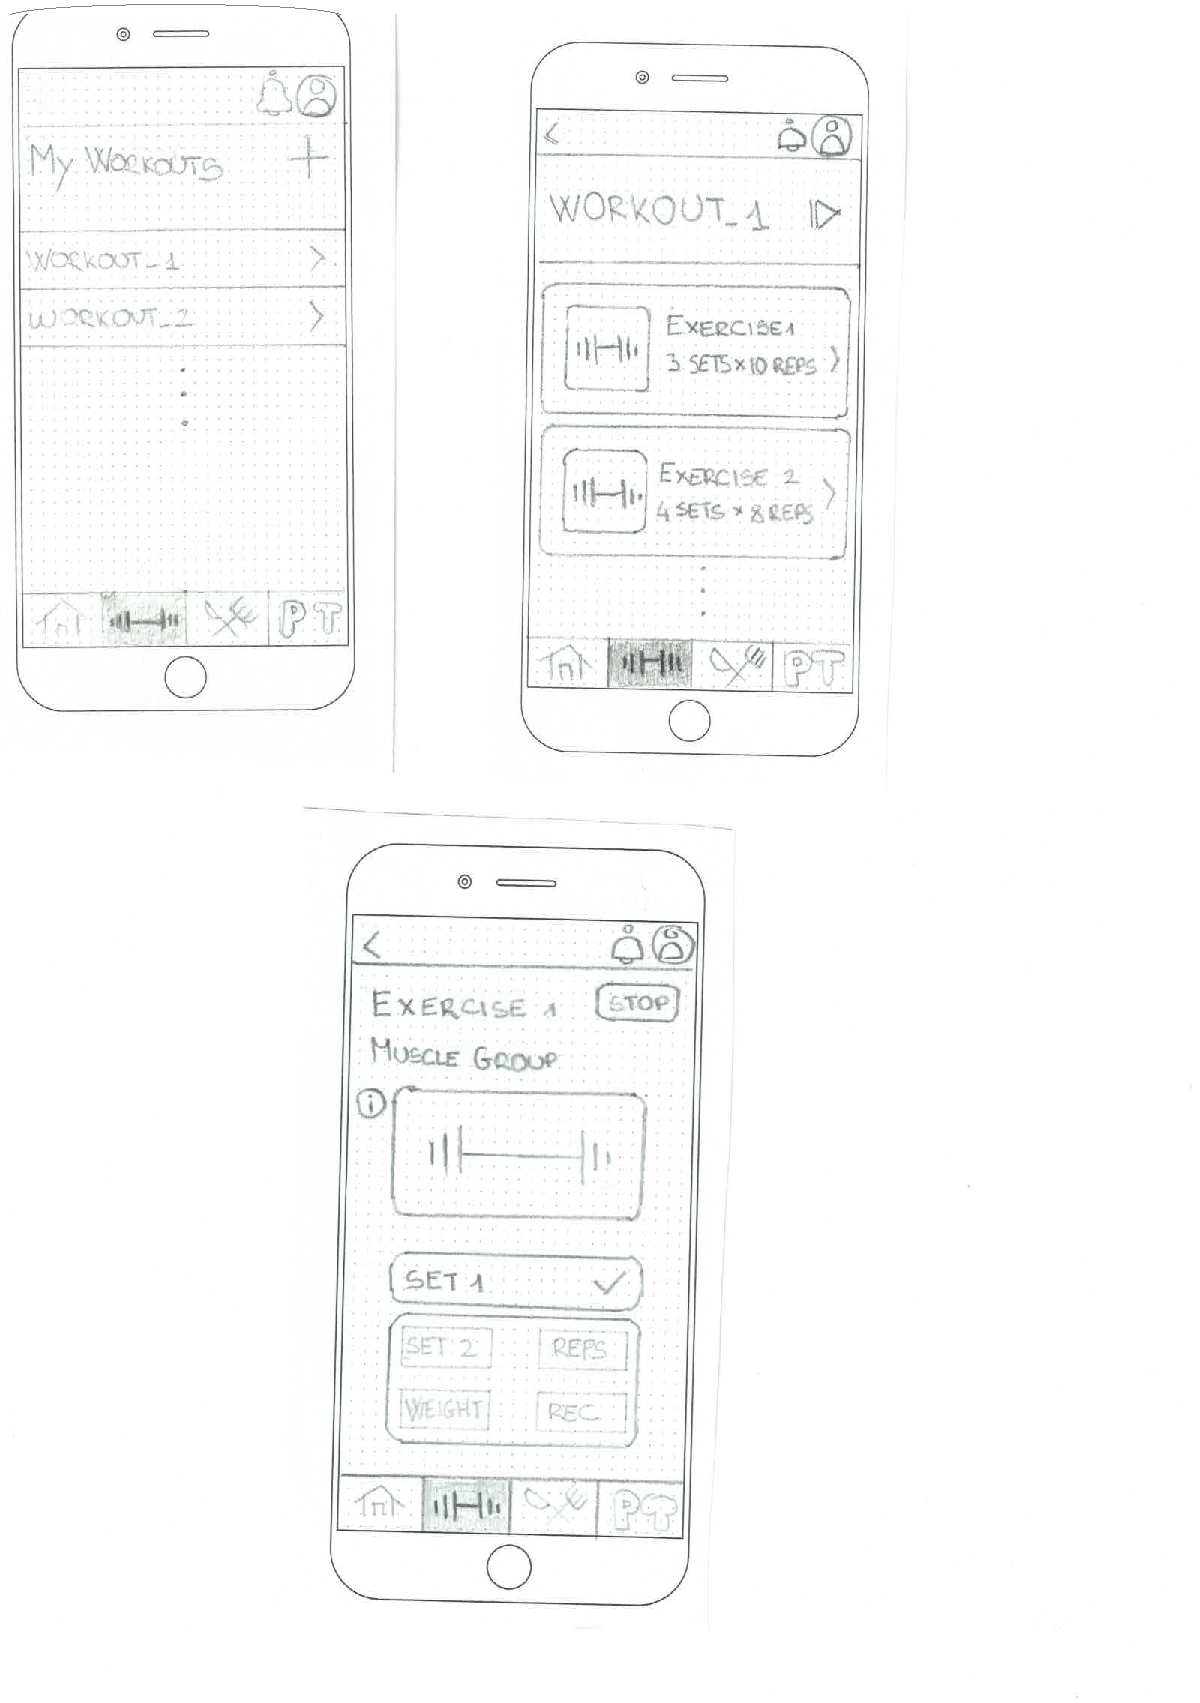
\includegraphics[width=0.62\textwidth]{4-ApplicationDesign/img/PaperPrototype/paper-member-workout-clean.pdf}
    \caption{Workout exploration and set recording.}
    \label{fig:paperMemberWorkout}
\end{figure}

\clearpage
\begin{figure}[H]
    \centering
    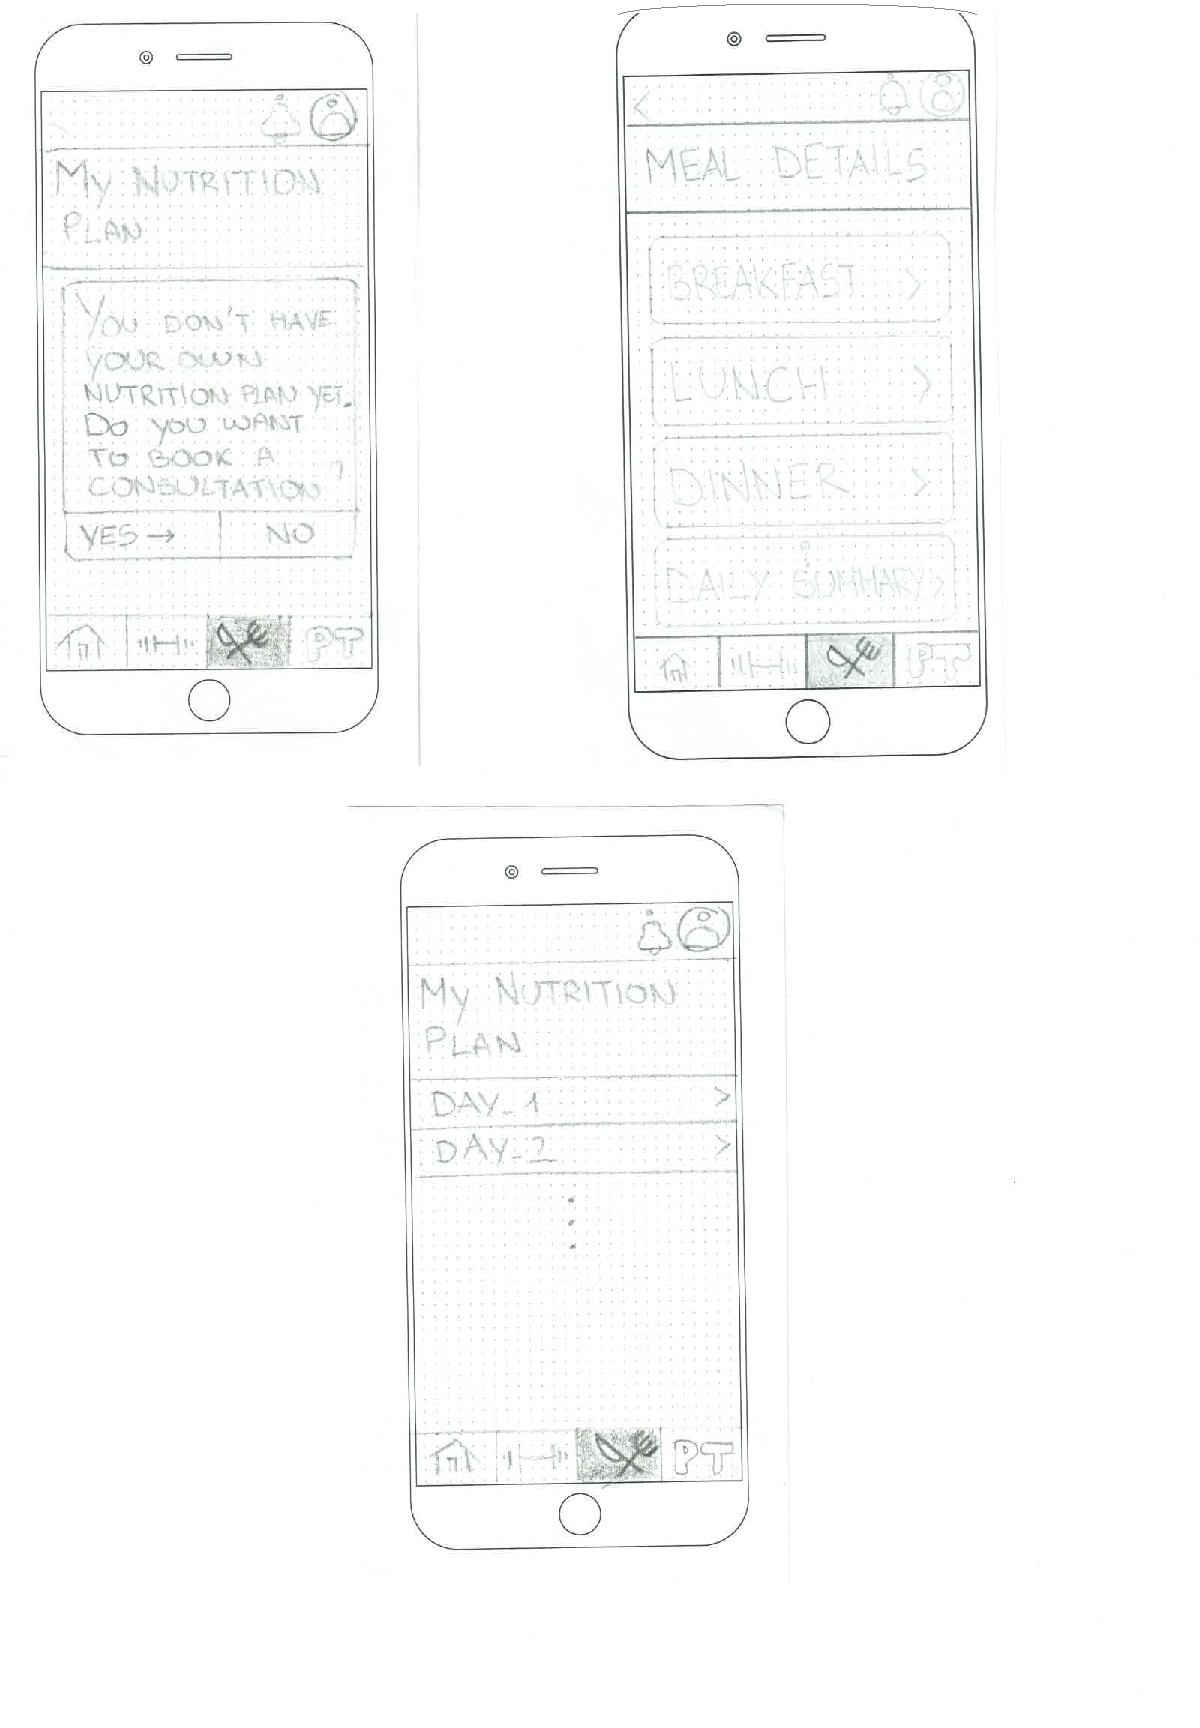
\includegraphics[width=0.80\textwidth]{4-ApplicationDesign/img/PaperPrototype/paper-member-nutrition-clean.pdf}
    \caption{Nutrition plan and meal details.}
    \label{fig:paperMemberNutrition}
\end{figure}

\clearpage
\begin{figure}[H]
    \centering
    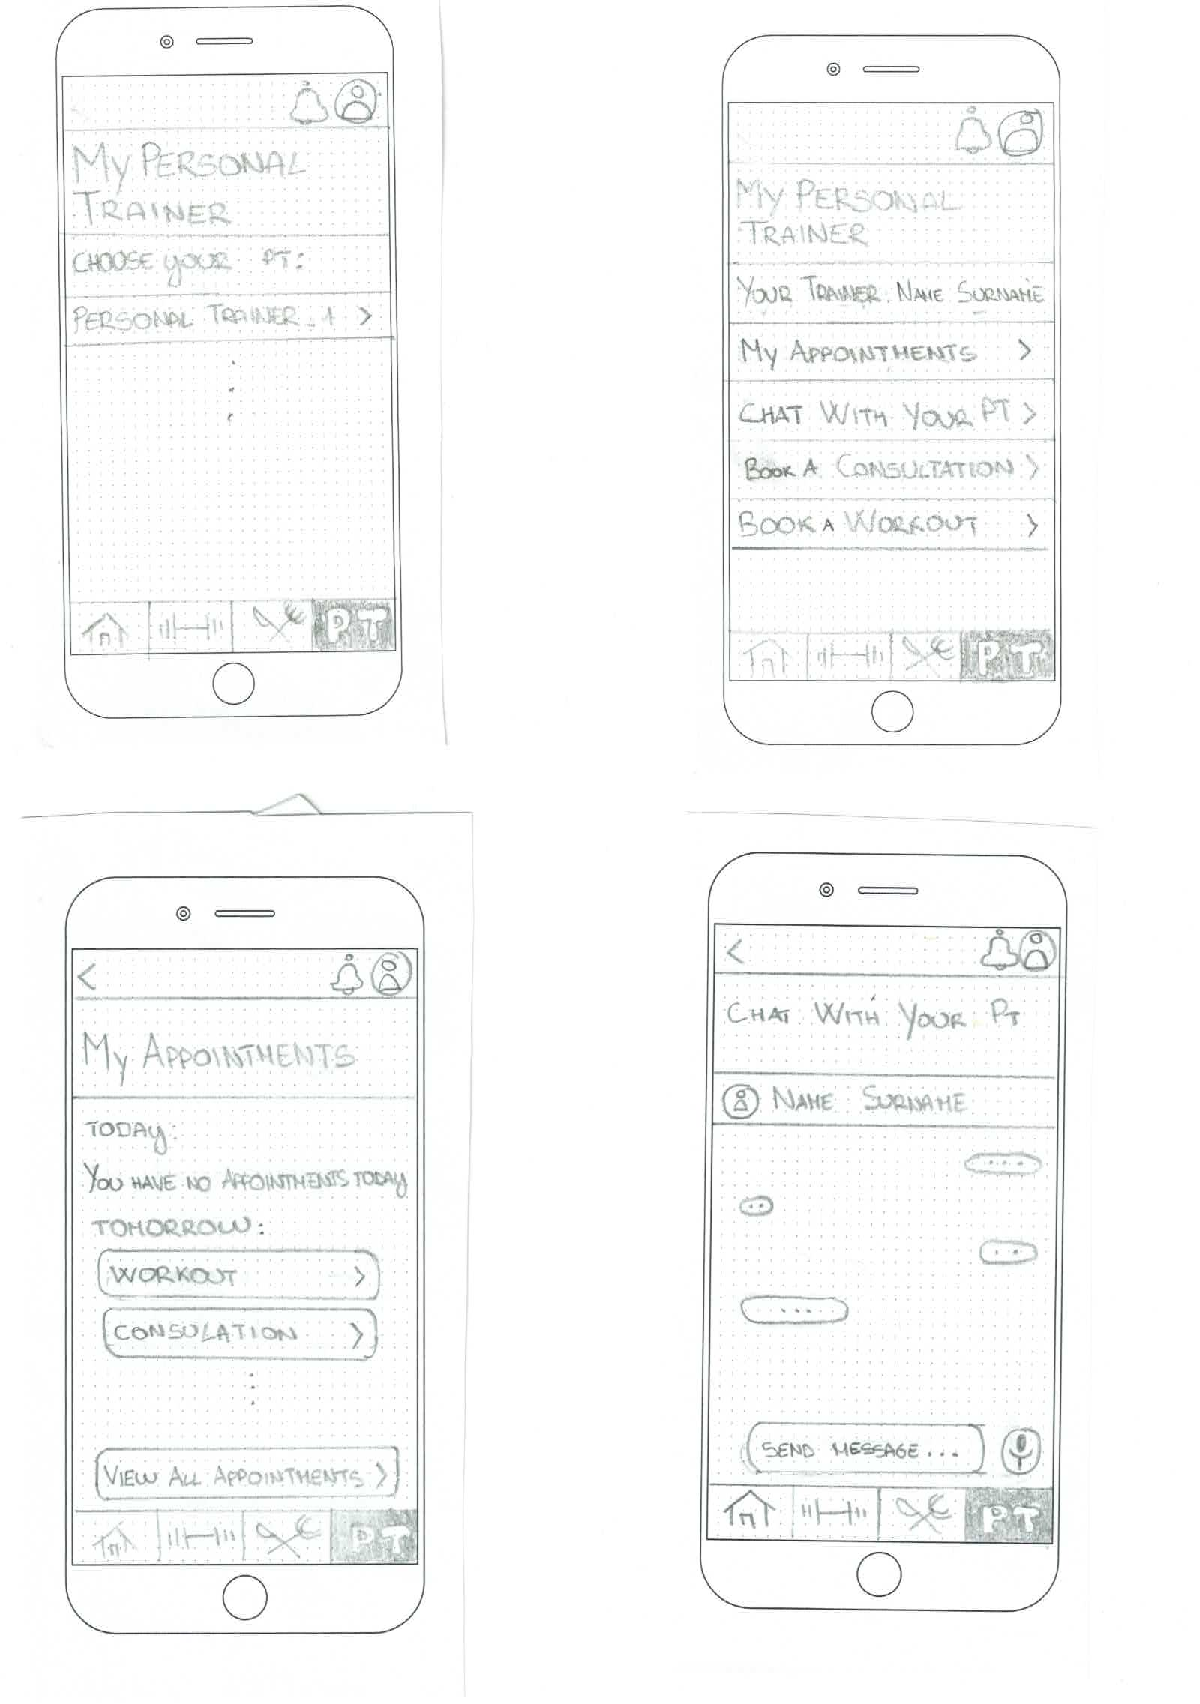
\includegraphics[width=0.80\textwidth]{4-ApplicationDesign/img/PaperPrototype/paper-member-trainer.pdf}
    \caption{Trainer selection, appointments, and chat.}
    \label{fig:paperMemberTrainer}
\end{figure}

\clearpage
\begin{figure}[H]
    \centering
    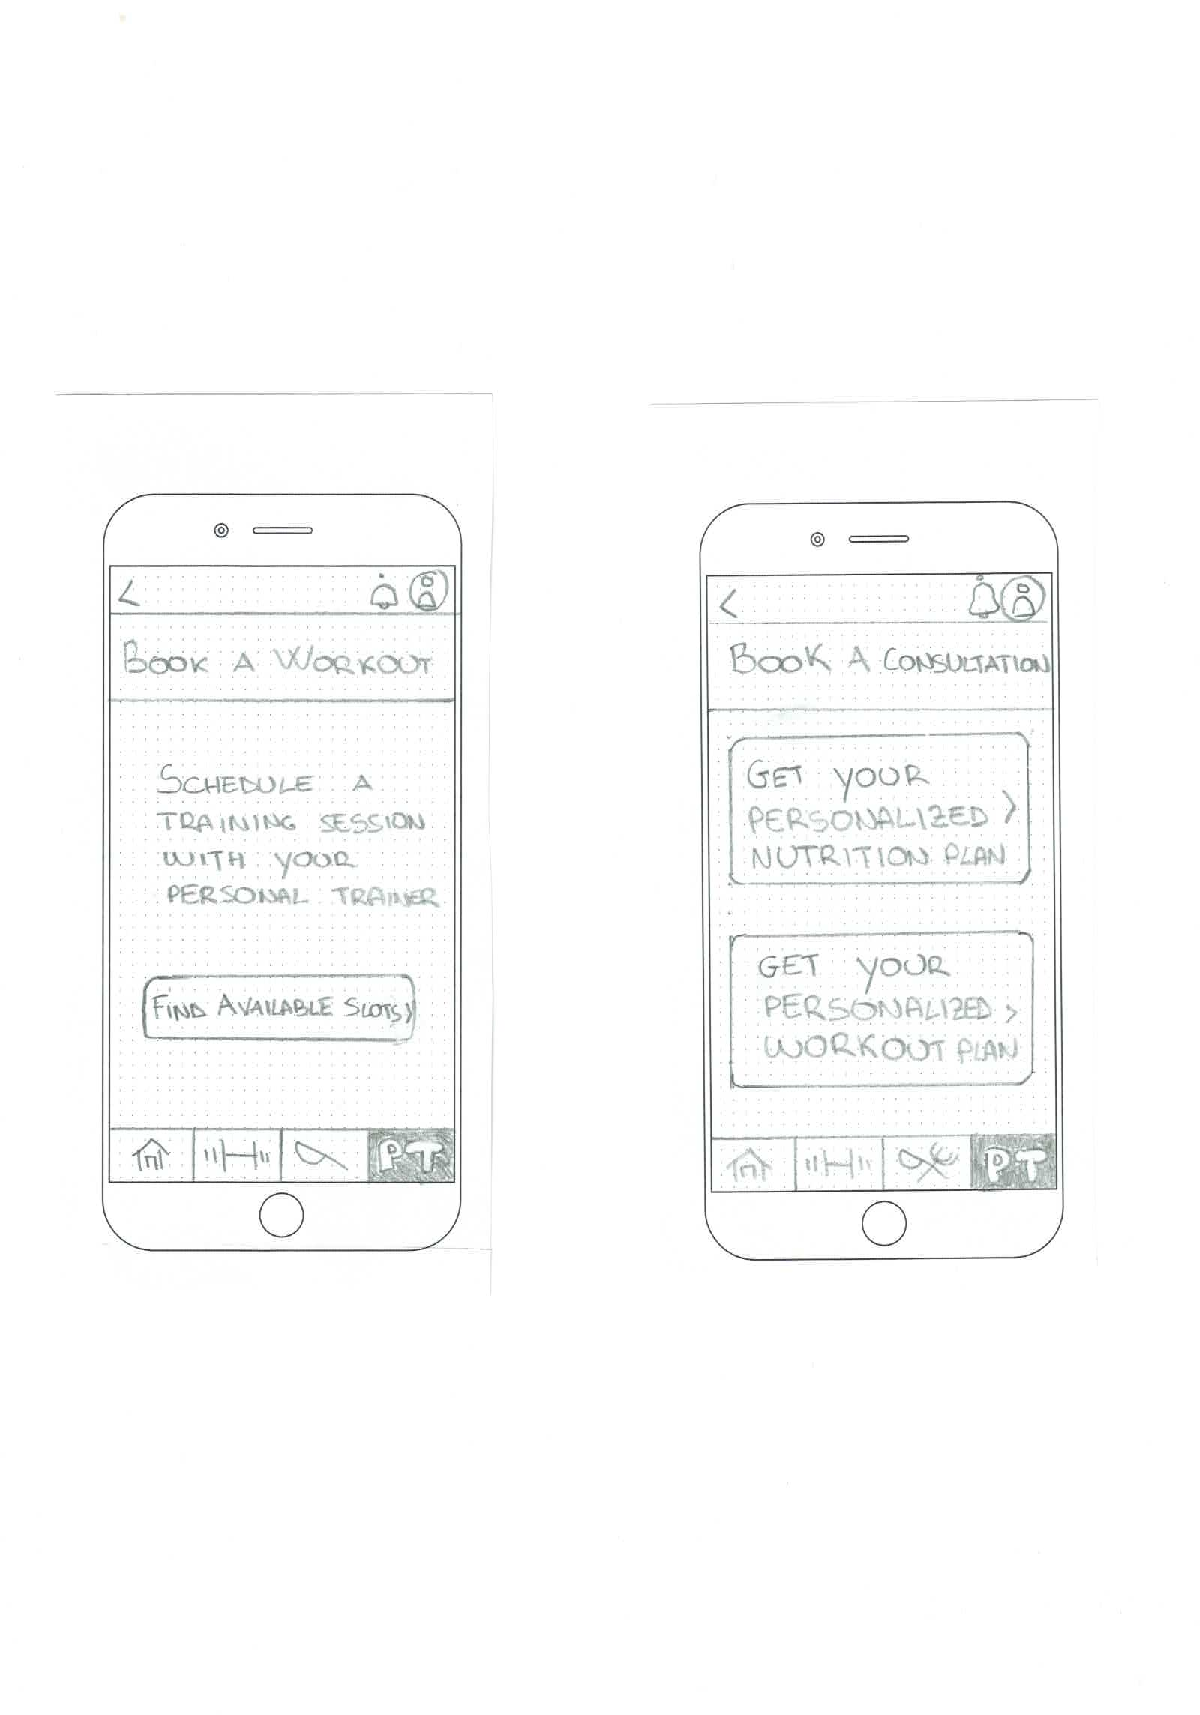
\includegraphics[width=0.72\textwidth,trim=18bp 175bp 34bp 165bp,clip]{4-ApplicationDesign/img/PaperPrototype/paper-member-booking.pdf}
    \caption{Booking entry points.}
    \label{fig:paperMemberBooking}
\end{figure}

\clearpage
\begin{figure}[H]
    \centering
    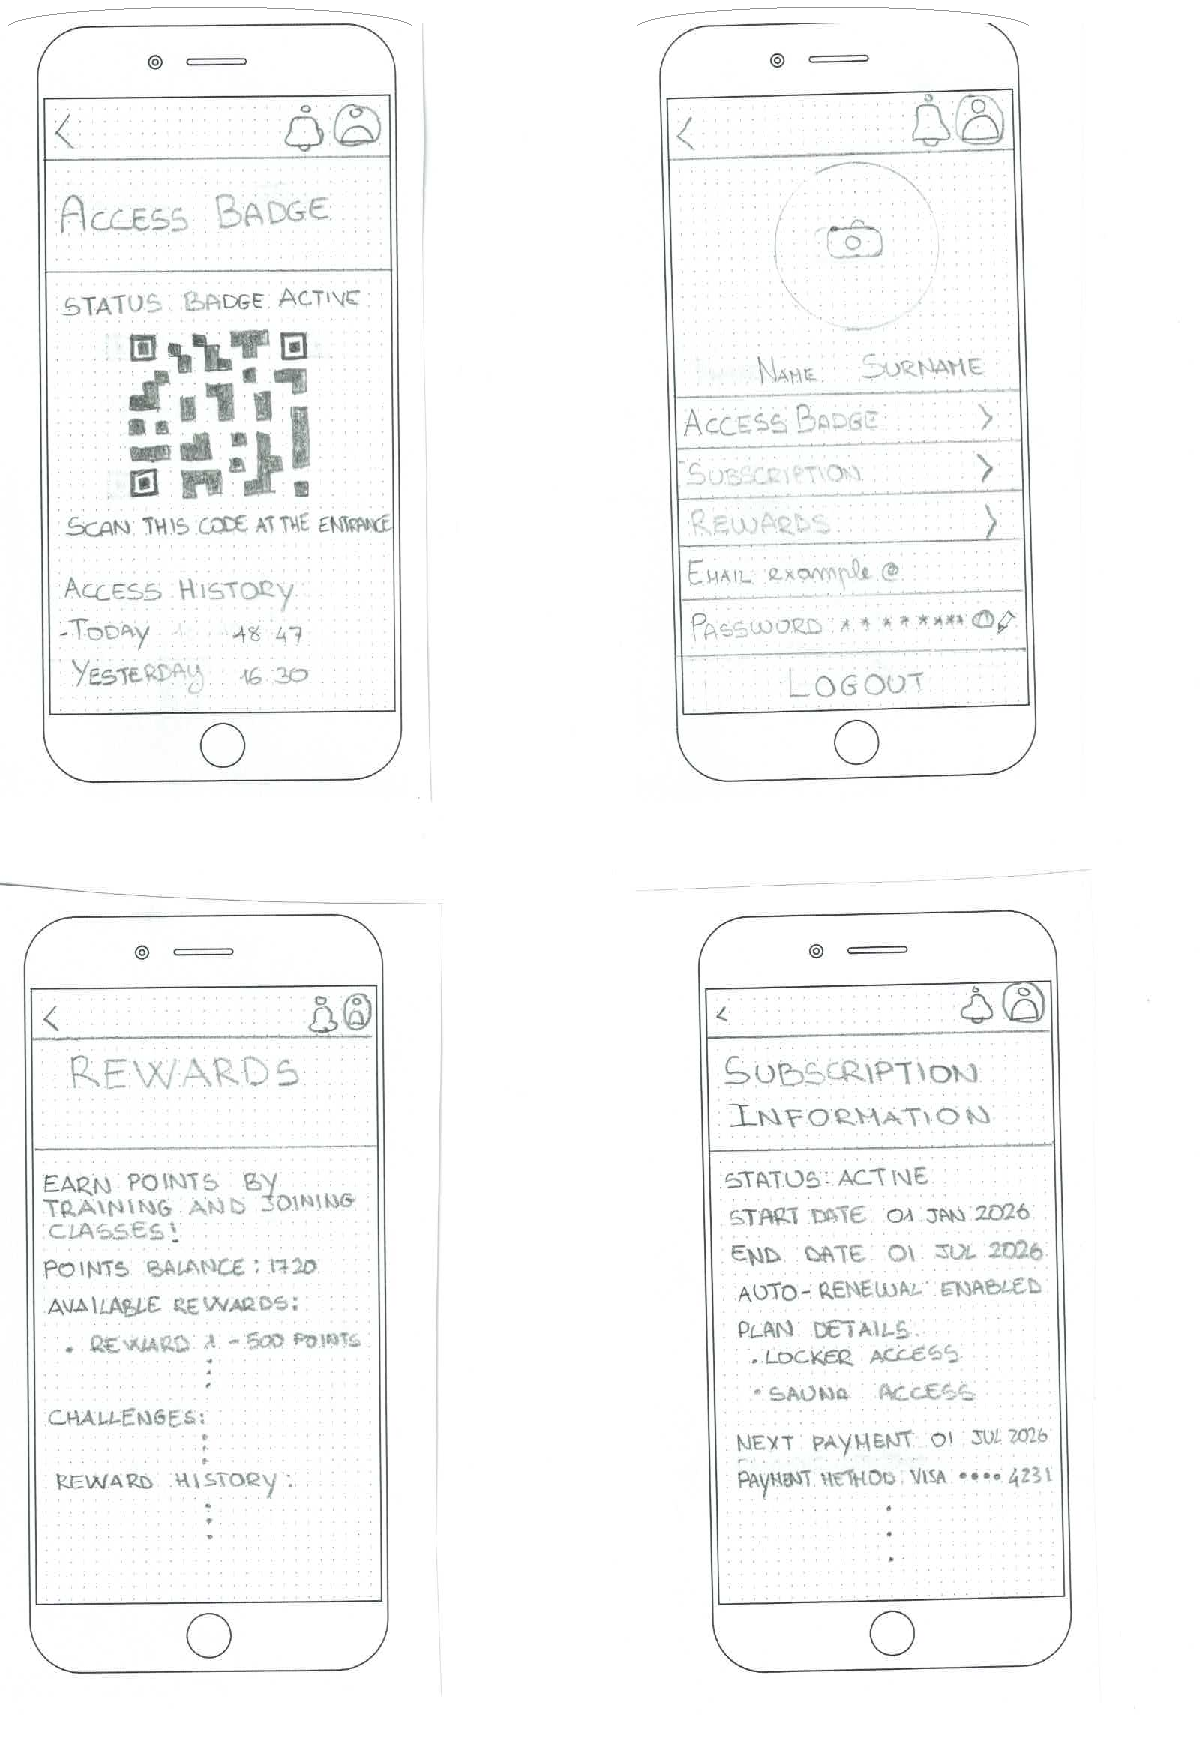
\includegraphics[width=0.80\textwidth]{4-ApplicationDesign/img/PaperPrototype/paper-member-profile-clean.pdf}
    \caption{Profile and membership.}
    \label{fig:paperMemberProfile}
\end{figure}

\clearpage
\paragraph{Professional Screens}

The professional sketches begin with the client list and use the selected client as the entry point for workout creation, nutrition management, progress, and appointments (Figure \ref{fig:paperProfessionalClients}). Profile, chat, and calendar remain independent destinations in the professional navigation (Figure \ref{fig:paperProfessionalScreens}).

\begin{figure}[H]
    \centering
    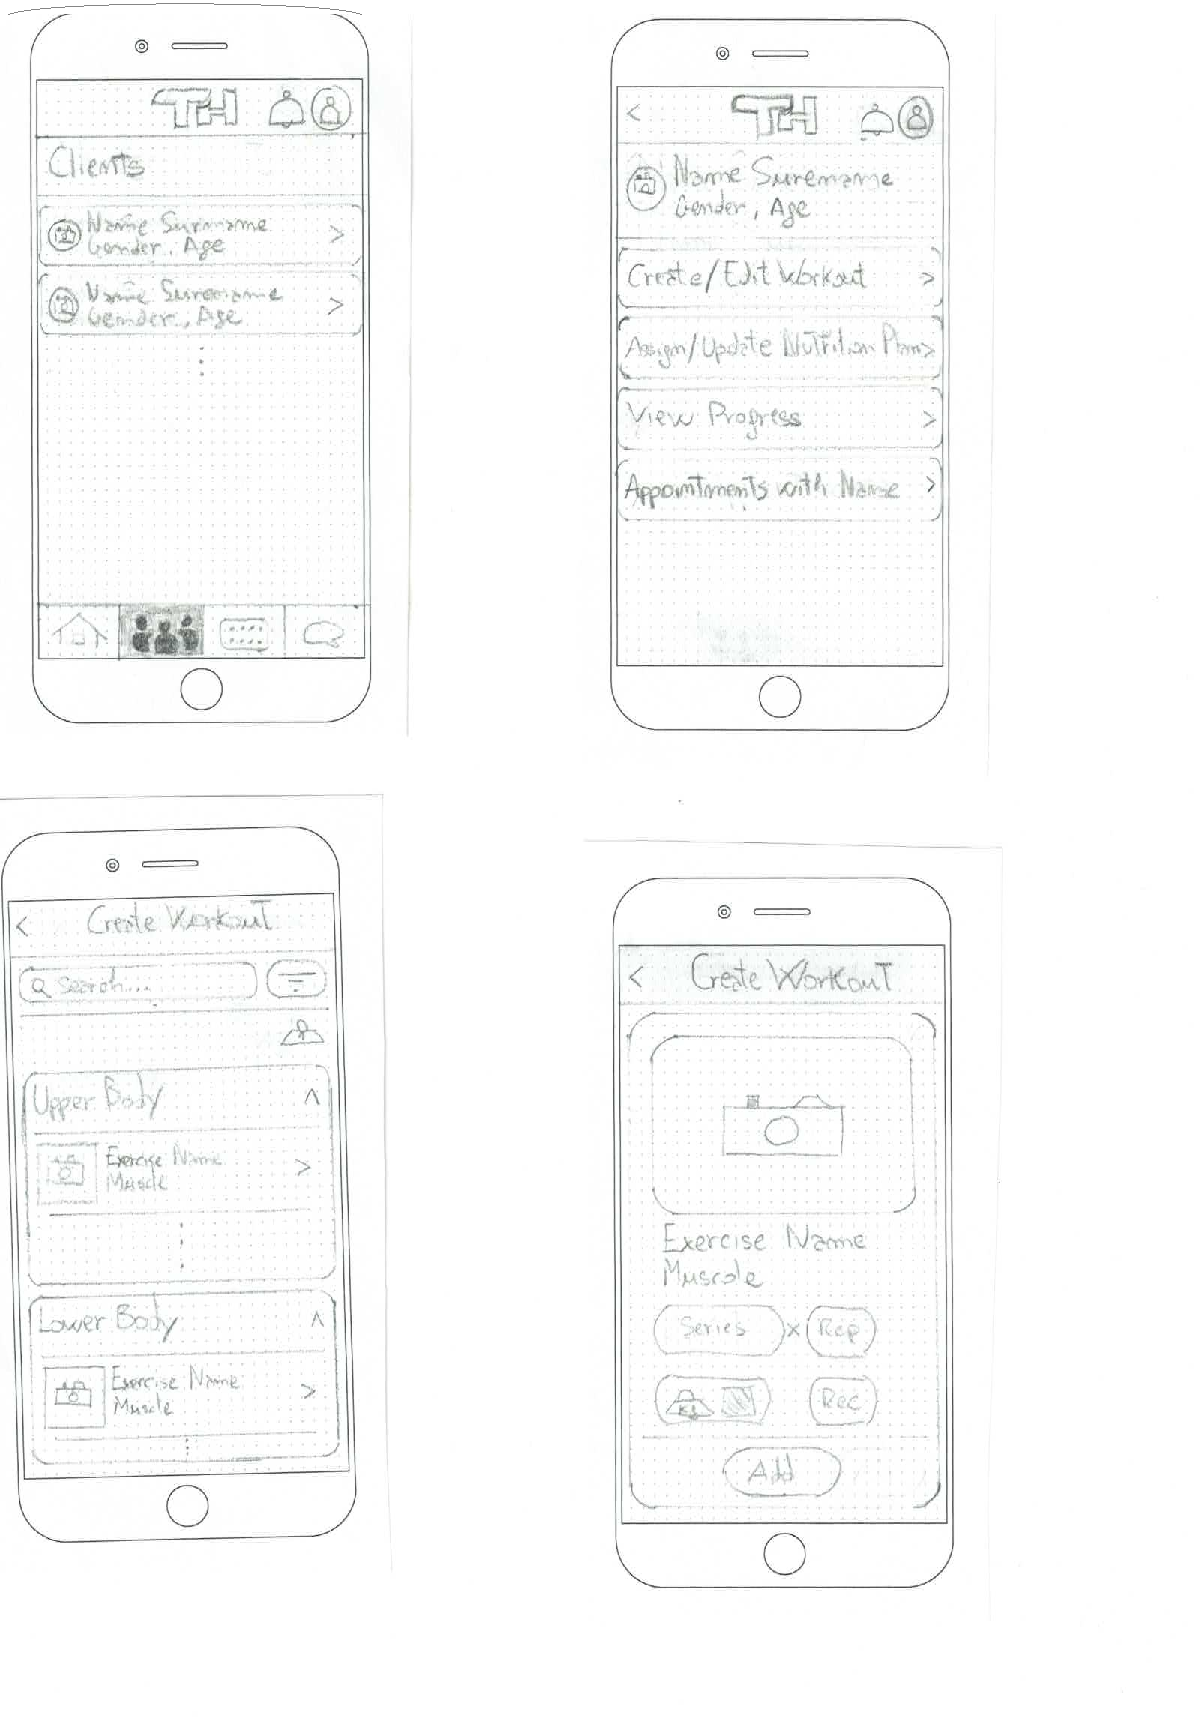
\includegraphics[width=0.56\textwidth]{4-ApplicationDesign/img/PaperPrototype/paper-professional-clients-clean.pdf}
    \caption{Client management and plan creation.}
    \label{fig:paperProfessionalClients}
\end{figure}

\clearpage
\begin{figure}[H]
    \centering
    \begin{subfigure}[b]{0.31\textwidth}
        \centering
        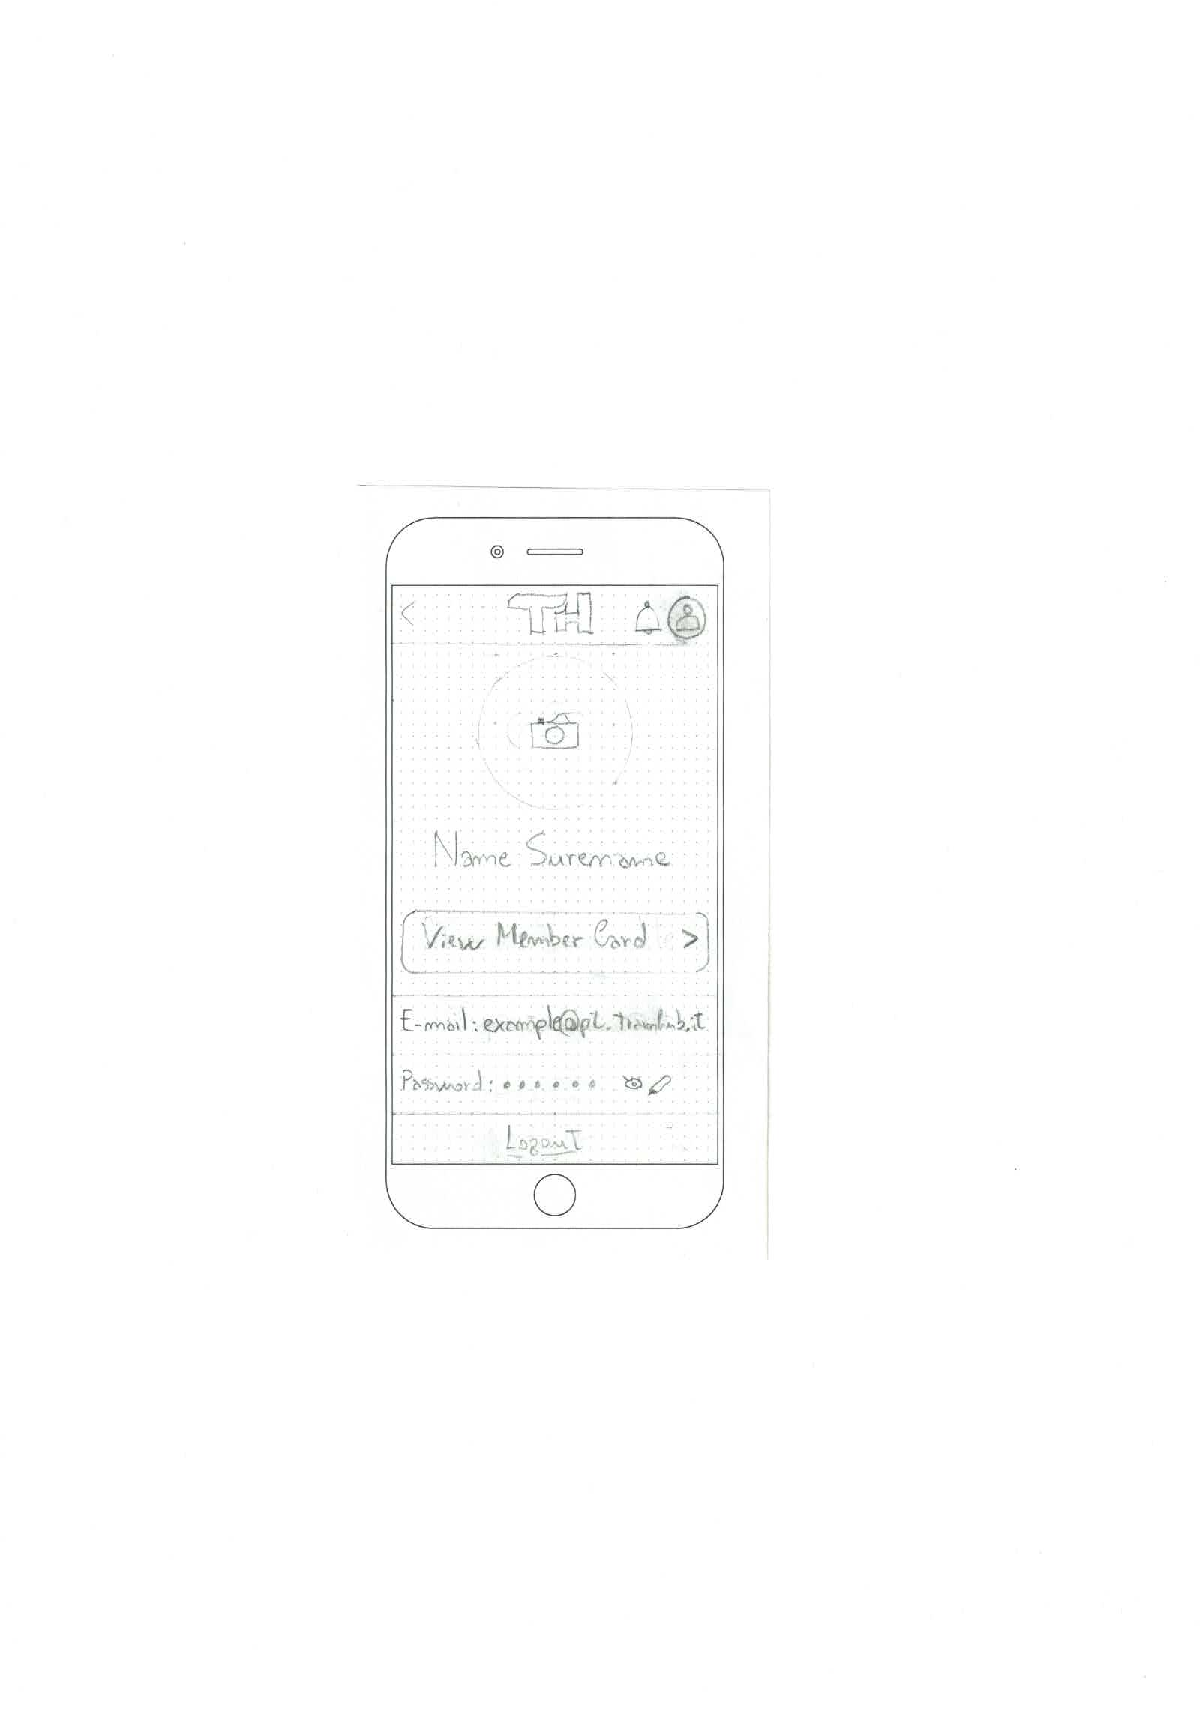
\includegraphics[height=7.5cm,keepaspectratio,trim=150bp 195bp 180bp 185bp,clip]{4-ApplicationDesign/img/PaperPrototype/paper-professional-profile.pdf}
        \caption{Profile.}
    \end{subfigure}
    \hfill
    \begin{subfigure}[b]{0.31\textwidth}
        \centering
        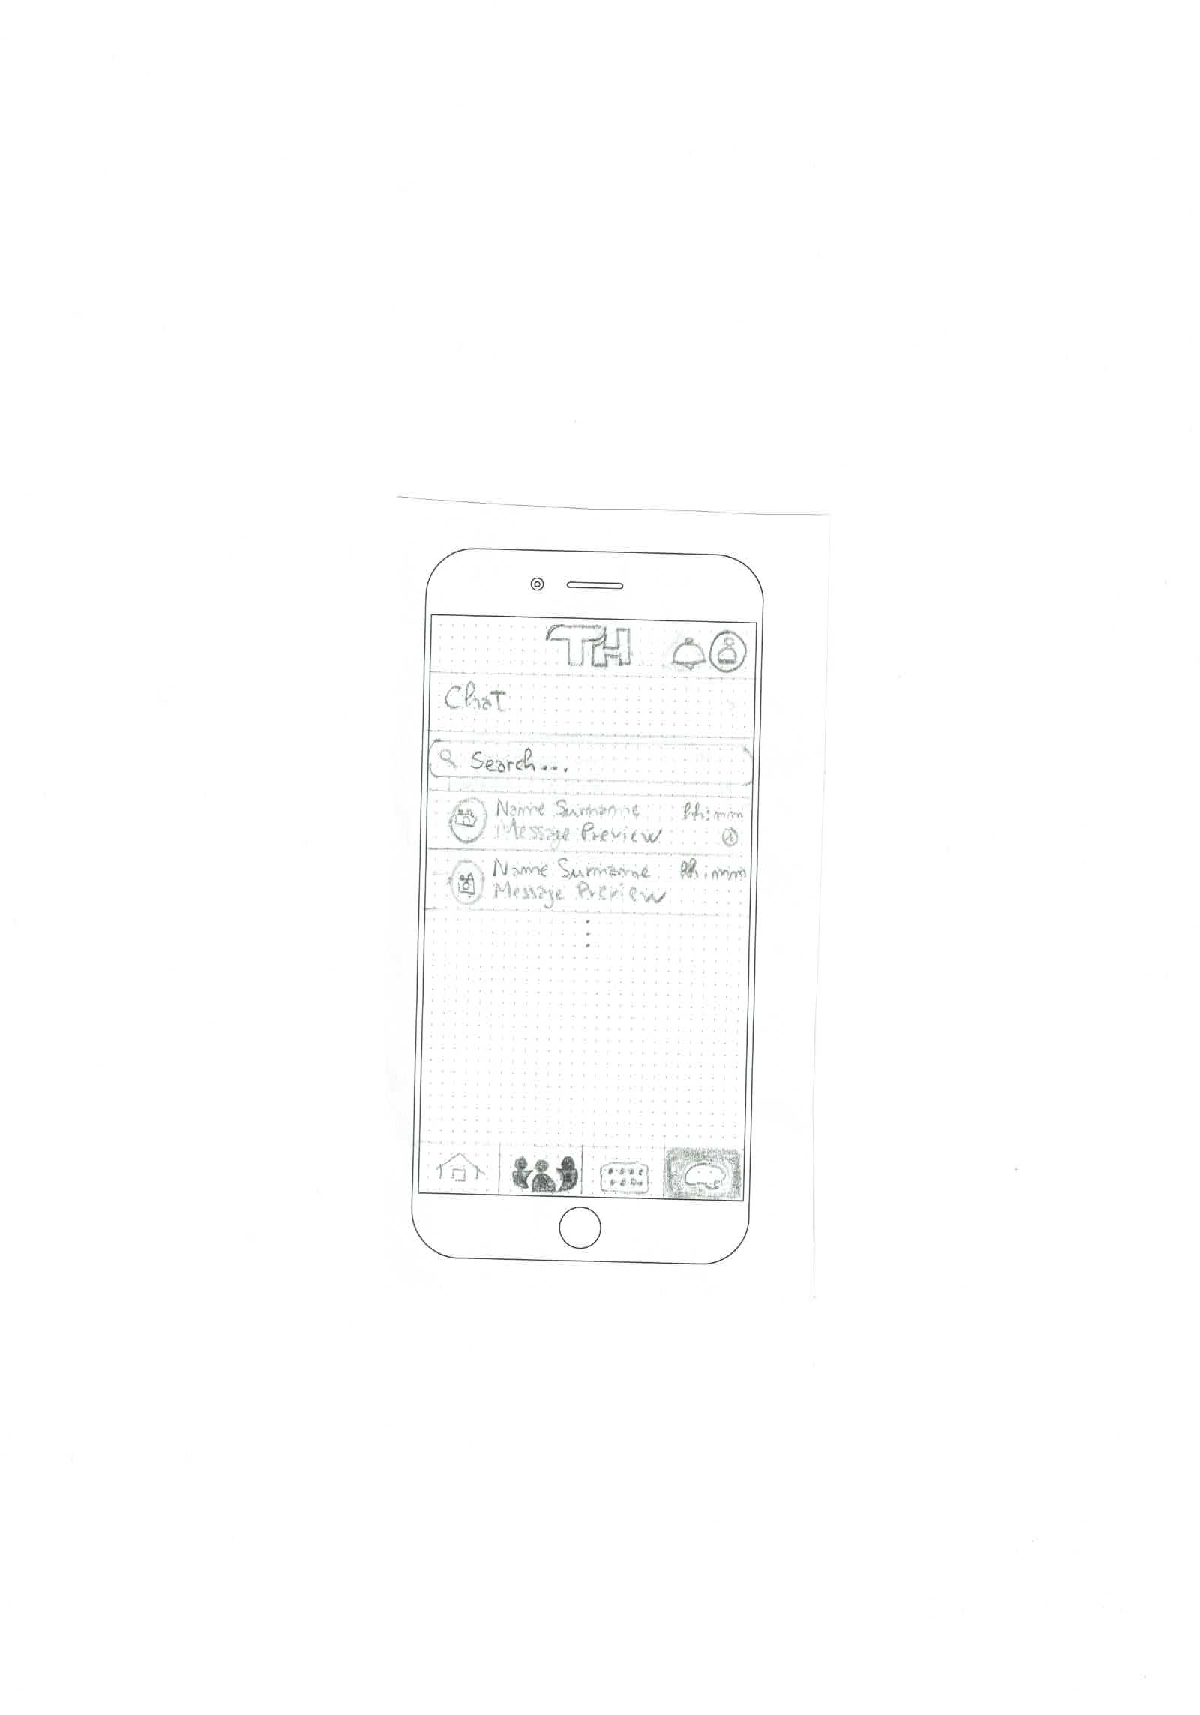
\includegraphics[height=7.5cm,keepaspectratio,trim=165bp 185bp 155bp 195bp,clip]{4-ApplicationDesign/img/PaperPrototype/paper-professional-chat.pdf}
        \caption{Chat.}
    \end{subfigure}
    \hfill
    \begin{subfigure}[b]{0.31\textwidth}
        \centering
        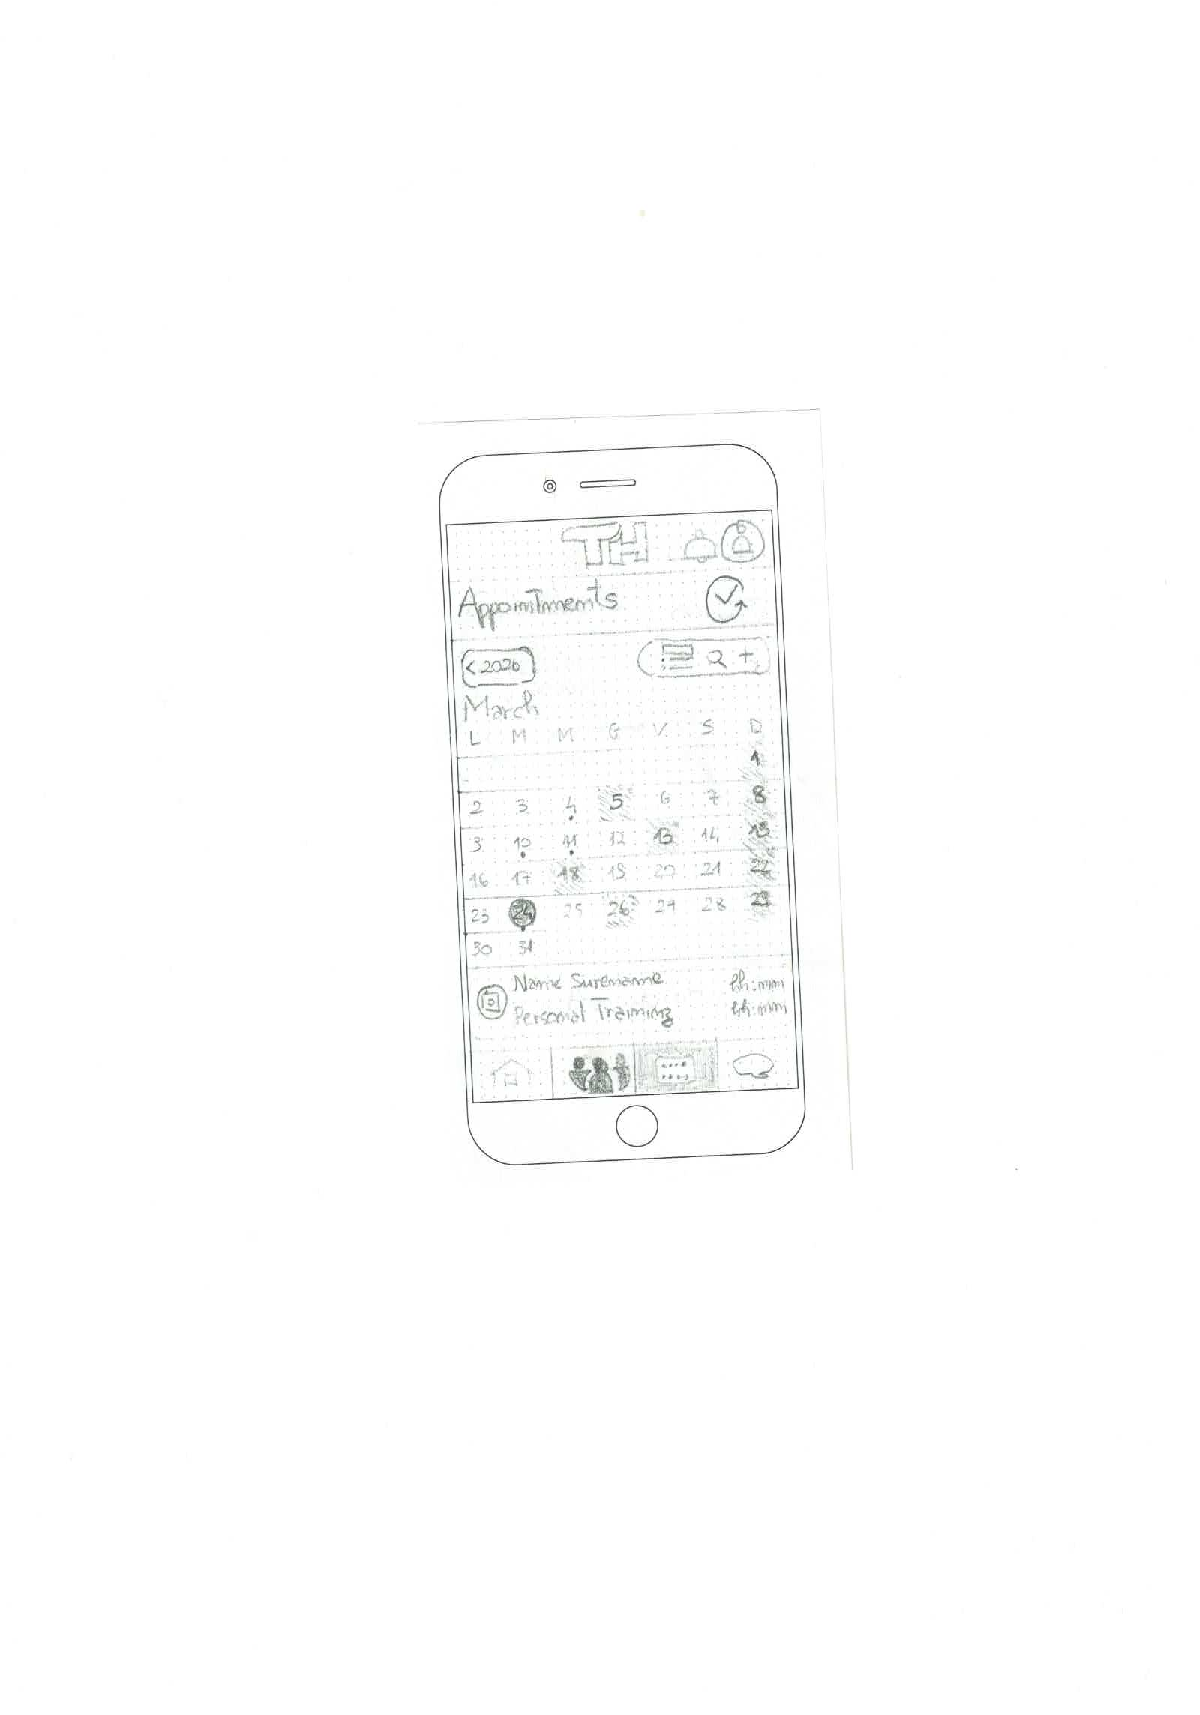
\includegraphics[height=7.5cm,keepaspectratio,trim=150bp 190bp 140bp 165bp,clip]{4-ApplicationDesign/img/PaperPrototype/paper-professional-calendar.pdf}
        \caption{Calendar.}
    \end{subfigure}
    \caption{The professional's independent destinations in the paper prototype.}
    \label{fig:paperProfessionalScreens}
\end{figure}

\clearpage
